\section{Introduction \& Application Motivation}
I am originally from Southern India, (in particular a city called Chennai), but when I go to visit my relatives who live in more remote parts of South India, I often hear stories about elephants wandering into villages and causing damage. I am also an Elephant enthusiast and have always been fascinated by these Elephants. This project is a way for me to combine my passion for elephants with real-world design considerations. 

\subsection{Background}
Elephants are a keystone species in the Indian subcontinent, playing a crucial role in forest ecosystems. However, human-elephant conflicts are a significant issue in regions where human settlements overlap with elephant habitats. Monitoring elephant migration patterns is essential for wildlife conservation and to mitigate human-elephant conflicts, as well as to preserve the Quality of Life for both humans and elephants. I localize my study to strictly Southern India to serve as a \textit{pilot} for a larger scale project that could be implemented in other parts of India and the world.

Figure \ref{fig:elephantmap} shows the current elephant migration patterns, especially concentrated in South India, which bolster the need for a system to monitor these elephants. The \textit{Annamadi}, \textit{Nilgiri}, and \textit{Periyar} while located in remote areas, are proximal to many important cities like \textbf{Bangalore}, \textbf{Coimbatore}, and \textbf{Madurai}, aggregating to a total population of over 20 million people\cite{elephantmap}. The need for a system to monitor these elephants is evident, and the system must be low-cost, low-power, and scalable to cover a large area.

\begin{figure}
    \centering
    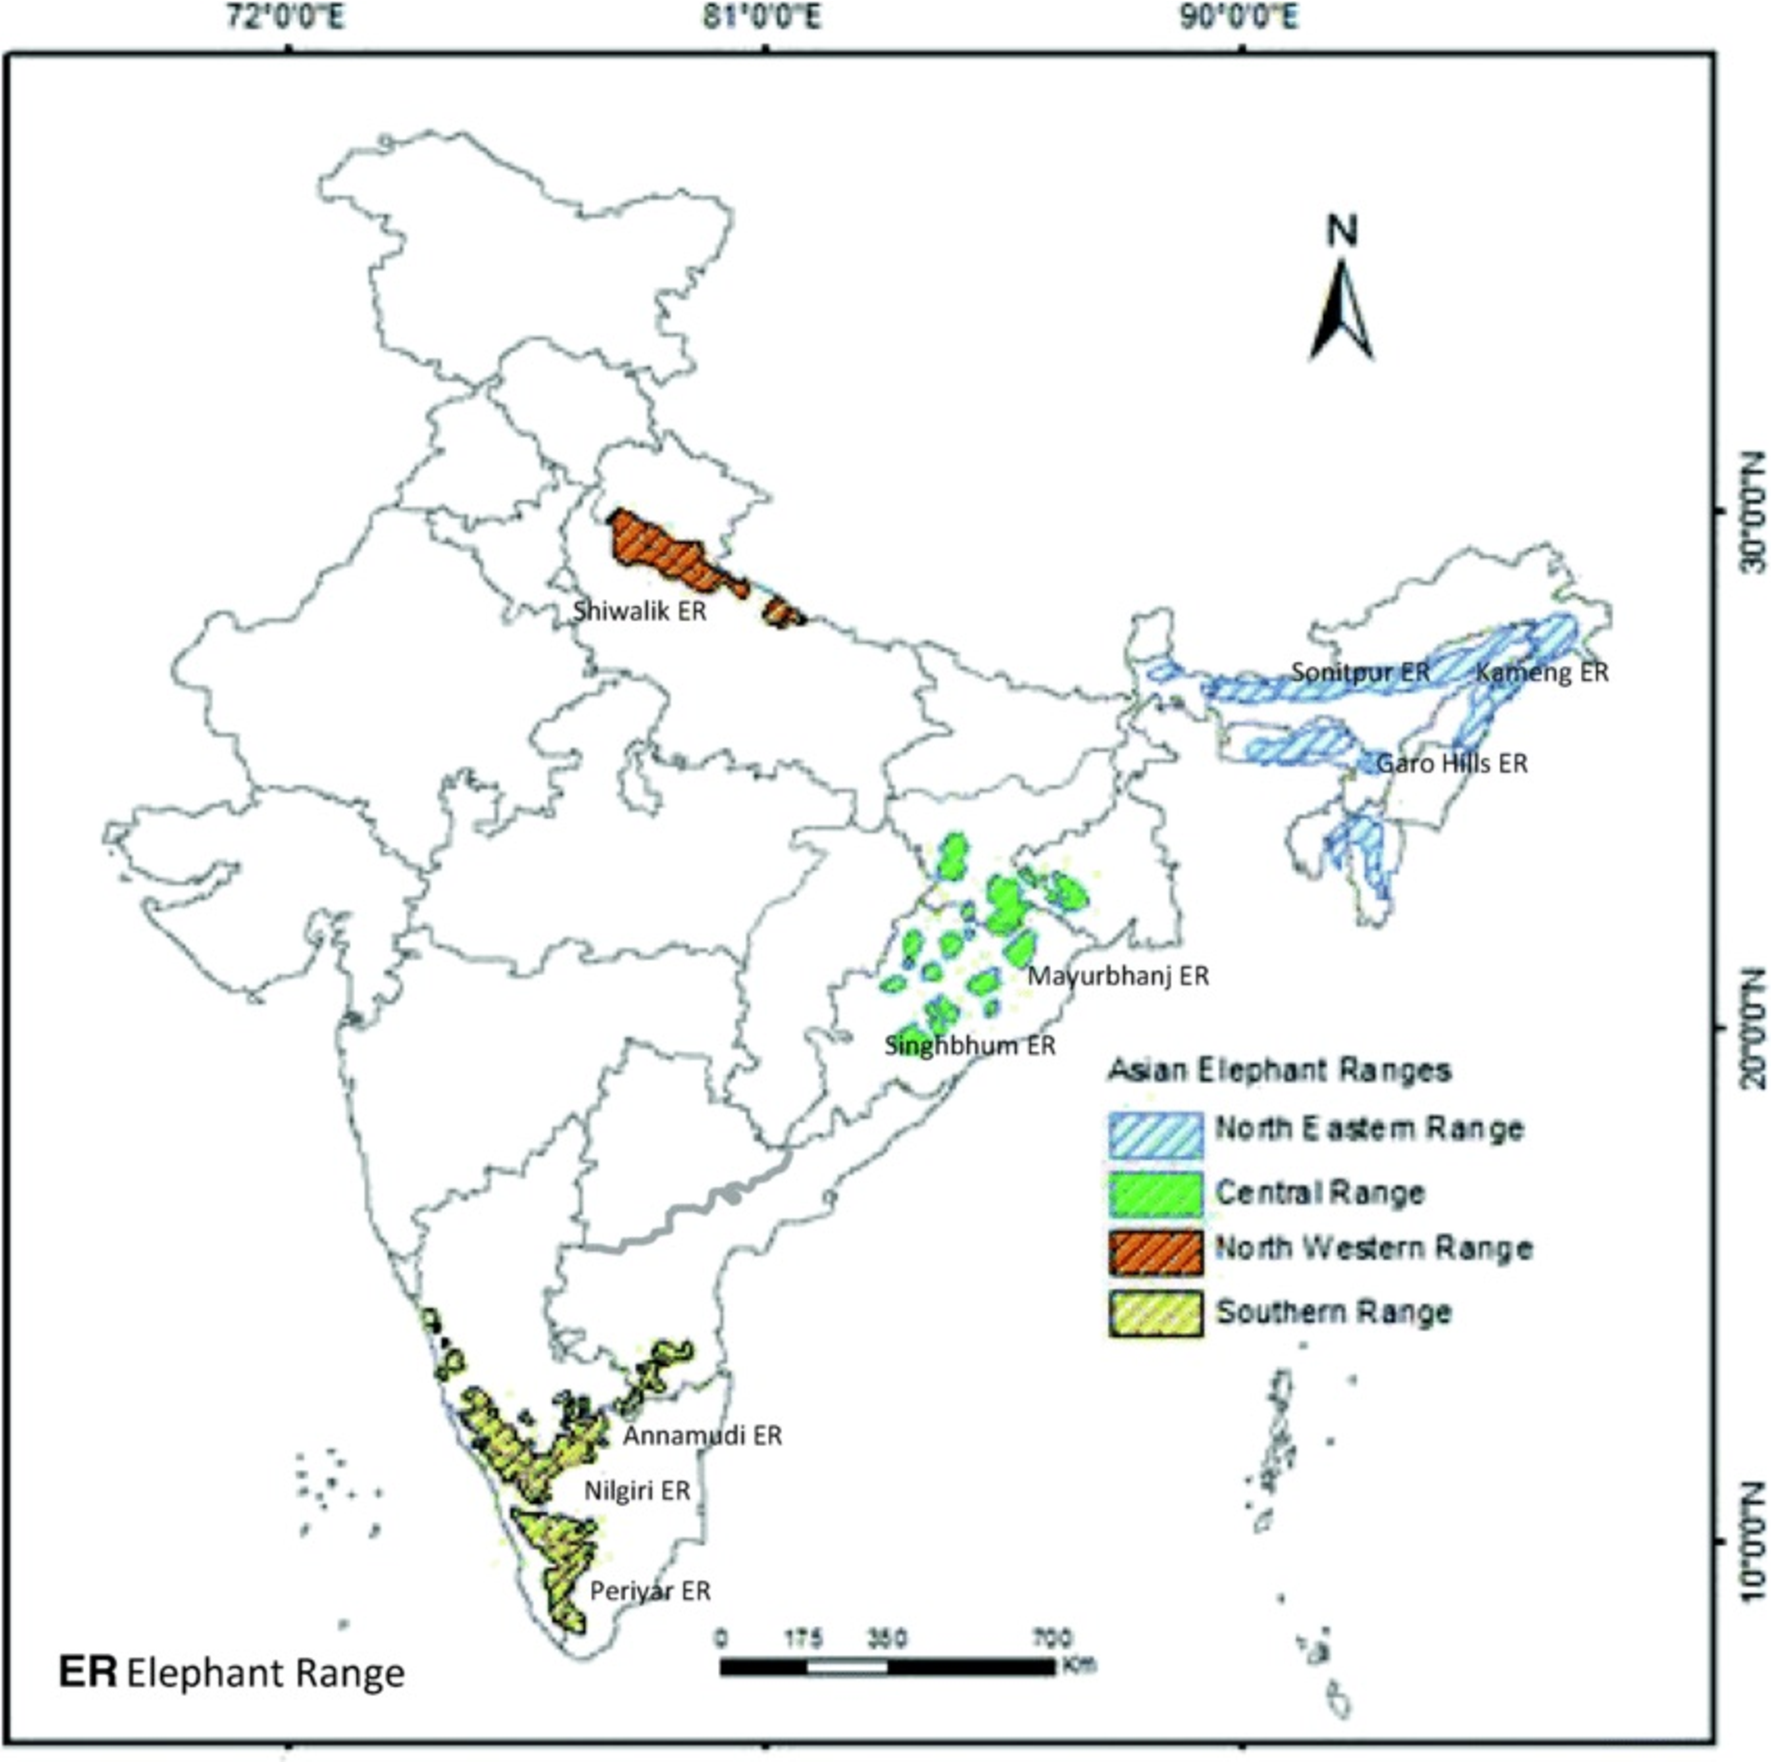
\includegraphics[width=0.9\columnwidth]{figures/Elephant-ranging-areas-in-India.pdf}
    \caption{Map of Current Elephant Migration Patterns and concentrated Habitats in India. Notice the concentration of elephants in the \textit{Annamadi}, \textit{Nilgiri}, and \textit{Periyar} Regions.}
    \label{fig:elephantmap}
\end{figure}

Also another important design consideration is the fact that the elephants habitat are spread in a variety of terrains, usually in high elevation, dense forests, and remote areas. This provides some road blocks in terms of connectivity and power, and also makes it difficult for large scale infrastructure to be built (i.e. cell phone towers, power lines, etc.). So relative to each sensor node, the system must be self-sufficient in terms of power for our pilot study, and must be able to communicate over long distances.

\begin{figure}
    \centering
    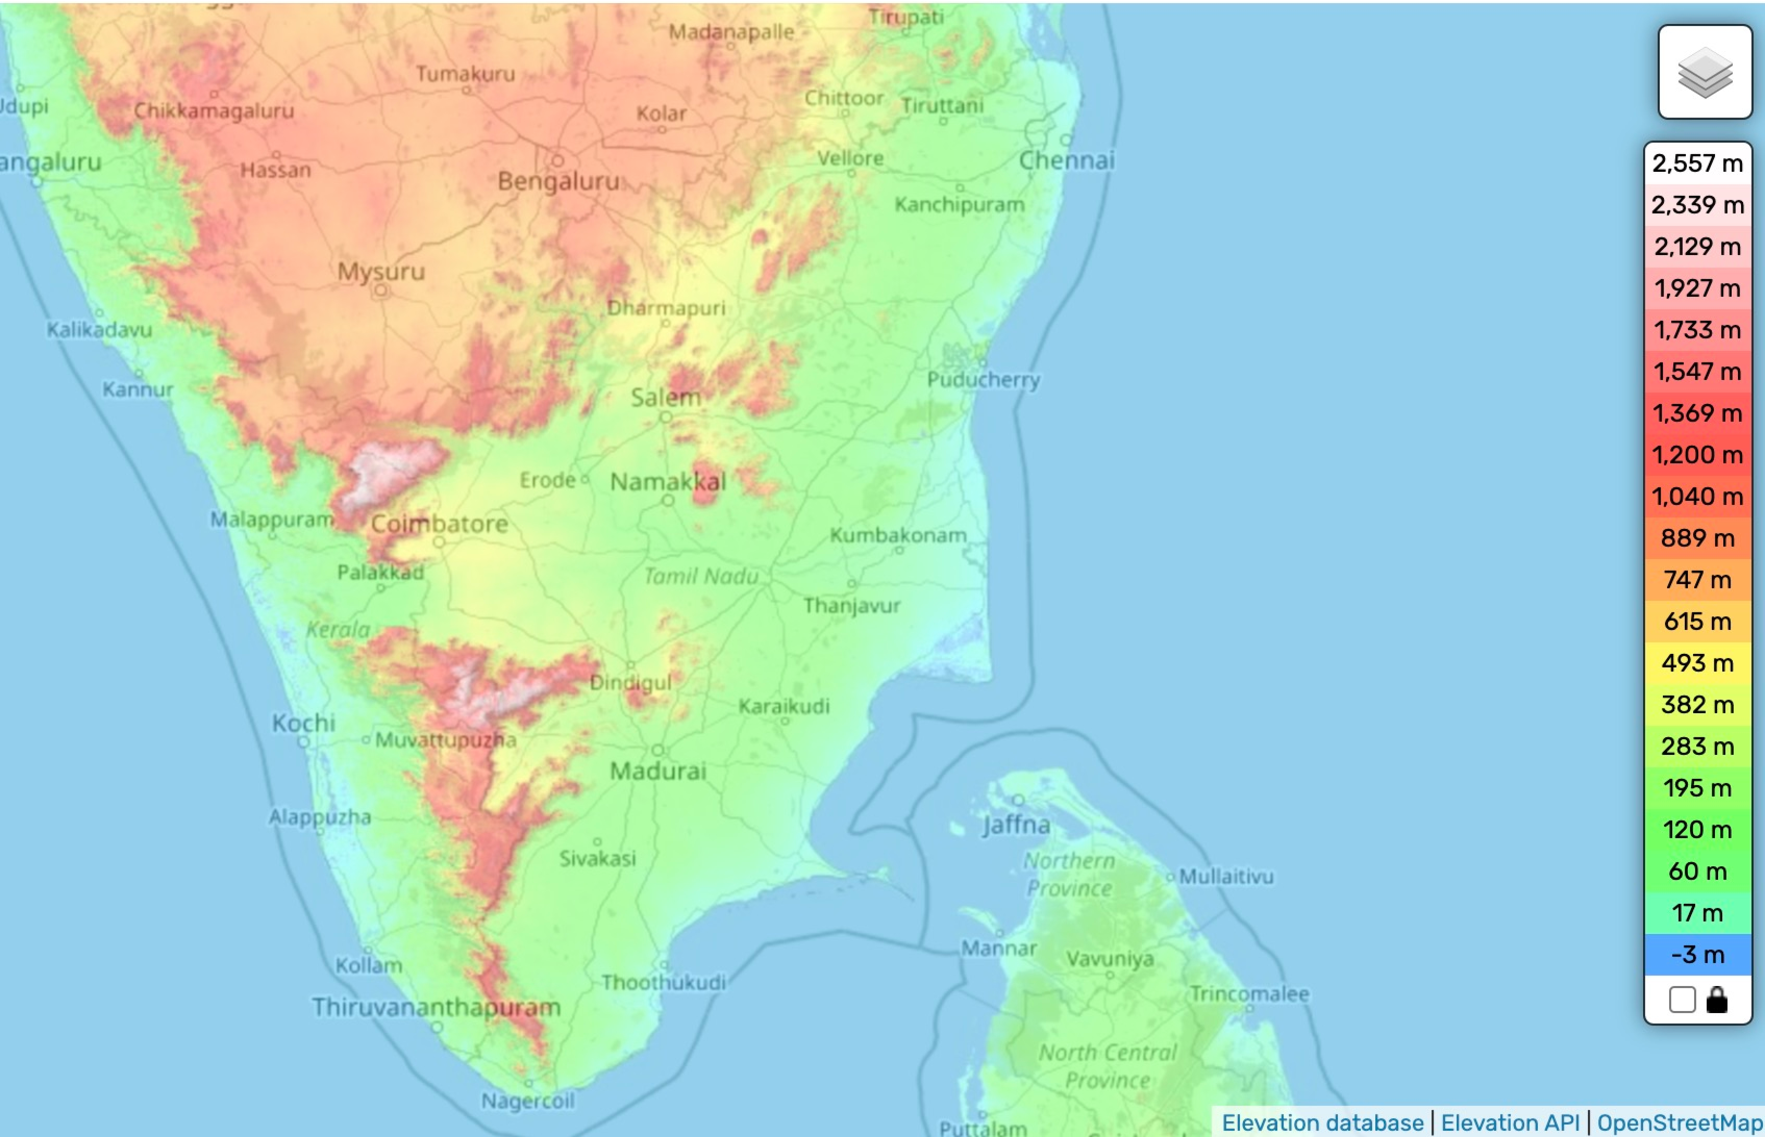
\includegraphics[width=0.9\columnwidth]{figures/GroundTopology.pdf}
    \caption{Ground Topology of the Elephant Habitat Area.}
    \label{fig:groundtopology}
\end{figure}